\chapter{Software Implementation Results}
\label{sec:aresults}

This chapter deals with the functional verification and execution time of the algorithm. The initial Matlab implementation is tried out with different pairs of stereo images and parameters to verify the functionality of the algorithm.  For this purpose BMPRE in DM in comparison with the ground truth is discussed. The outputs obtained are presented. Next, the run-time performance of various optimised versions of the C++ implementation across different hardware is discussed. Images from Tsukuba university \cite{Martull2012,Peris2012} and Middlebury university \cite{Scharstein2001,Scharstein2003} are used for the purpose of evaluation.
%

%%%%%%%%%%%%%%%%%%%%%%%%%%%%%%%%%%%%%
%%%%%%%%%%%%%%%%%%%%%%%%%%%%%%%%%%%%%
%%%%%%%%%%%%   SECTION   %%%%%%%%%%%%
%%%%%%%%%%%%%%%%%%%%%%%%%%%%%%%%%%%%%
%%%%%%%%%%%%%%%%%%%%%%%%%%%%%%%%%%%%%
\section{Parameters}
\label{sec:parameters}

The important parameters which determine the quality of the DM, and the run time of the selected algorithm are, \begin{itemize}
\item{The morphological opening window size (MW)}
\item{The census transform window size (CTW)}
\item{The range od disparity values (D range)}
\item{The SHD window size (SHDW)}
\end{itemize}

These parameters are varied among a range of values and the corresponding functionality of the algorithm is recorded. An optimal set of parameters from is chosen for the eGPU evaluation.

%%%%%%%%%%%%%%%%%%%%%%%%%%%%%%%%%%%%%
%%%%%%%%%%%%%%%%%%%%%%%%%%%%%%%%%%%%%
%%%%%%%%%%%%   SECTION   %%%%%%%%%%%%
%%%%%%%%%%%%%%%%%%%%%%%%%%%%%%%%%%%%%
%%%%%%%%%%%%%%%%%%%%%%%%%%%%%%%%%%%%%
\section{Functional verification results}
\label{sec:fverificationres}

The BMPRE method described in the Section \ref{s:stereovision:bmpre} is used for functional verification. In this section, the parameter values are varied and the corresponding BMPRE values are observed. The values giving the least BMPRE are chosen for the eGPU implementation.

%%%%%%%%%%%%%%%%%%%%%%%%%
%%%%%   SUB-SECTION   %%%
%%%%%%%%%%%%%%%%%%%%%%%%%
%%%%%%%%%%%%%%%%%%%%%%%%%
\subsection{Morphological opening window size (MW)}
\label{s:fverificationres:mw}

\begin{figure}
  \center
  \captionsetup{justification=centering}
  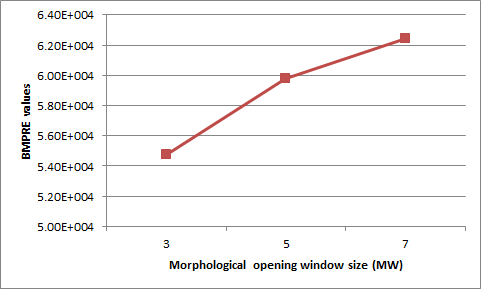
\includegraphics[width=.8\linewidth]{figures/BMPRE1}
  \caption{BMPRE values ($\delta$=2) across different MW values. Other parameters are kept constant with CTW=11, D range: 0-100, and SHDW=13}
  \label{fig:bmpre1}
\end{figure}


The Section \ref{s:algorithm:preprocessing} explains about the morphological opening operation. Different MW values are experimented while keeping the other parameters constant, and the BMPRE values are observed. In this experiment CTW is 11, D range ranges from 0 to 100, and SHDW is 13. The first frame of Tsukuba university image pair is chosen for evaluation. As indicated in the Section \ref{s:stereovision:bmpre} $\delta$ value is kept at 2. The results for MW values 3,5, and 7 are as shown in the Figure \ref{fig:bmpre1}. It can be seen that MW value of 3 yields the best results.

\subsection{Census transform window size (CTW) and disparity range (D range)}
\label{s:fverificationres:mw}

\begin{figure}
\captionsetup[subfigure]{justification=centering}
\begin{subfigure}{.5\textwidth}
  \centering
  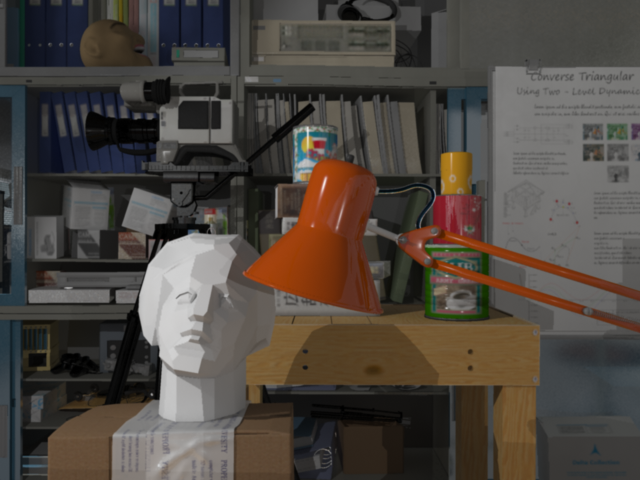
\includegraphics[width=.8\linewidth]{figures/frame_1_right}
  \caption{Original image (right)}
  \label{fig:sfig1}
\end{subfigure}
\begin{subfigure}{.5\textwidth}
  \centering
  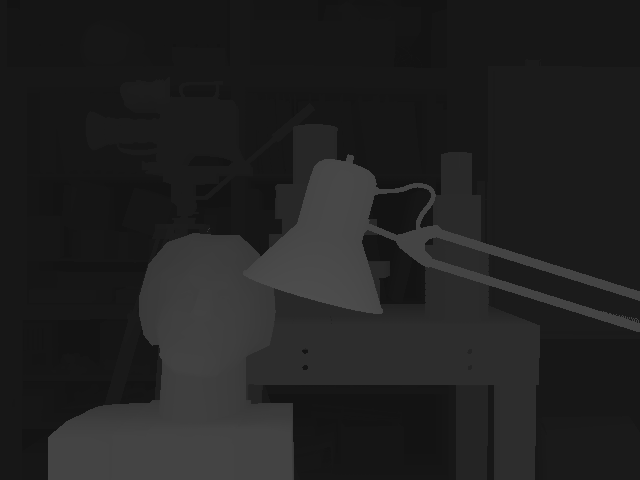
\includegraphics[width=.8\linewidth]{figures/frame_1}
  \caption{Ground truth}
  \label{fig:sfig2}
\end{subfigure}
\begin{subfigure}{.5\textwidth}
  \centering
  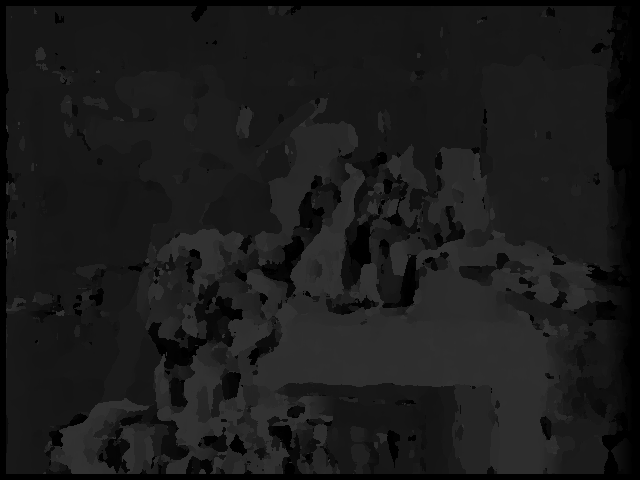
\includegraphics[width=.8\linewidth]{figures/CT7D0-50}
  \caption{7x7 census transform window \\Disparity range 0 to 50}
  \label{fig:sfig3}
\end{subfigure}%
\begin{subfigure}{.5\textwidth}
  \centering
  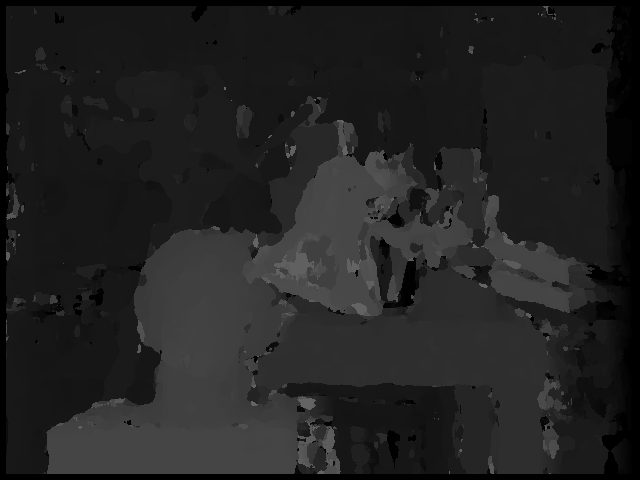
\includegraphics[width=.8\linewidth]{figures/CT7D0-100}
  \caption{7x7 census transform window \\Disparity range 0 to 100}
  \label{fig:sfig4}
\end{subfigure}
\begin{subfigure}{.5\textwidth}
  \centering
  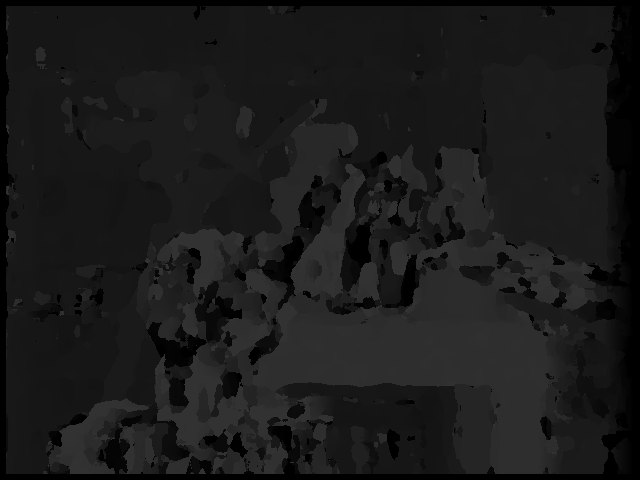
\includegraphics[width=.8\linewidth]{figures/CT9D0-50}
  \caption{9x9 census transform window \\Disparity range 0 to 50}
  \label{fig:sfig5}
\end{subfigure}%
\begin{subfigure}{.5\textwidth}
  \centering
  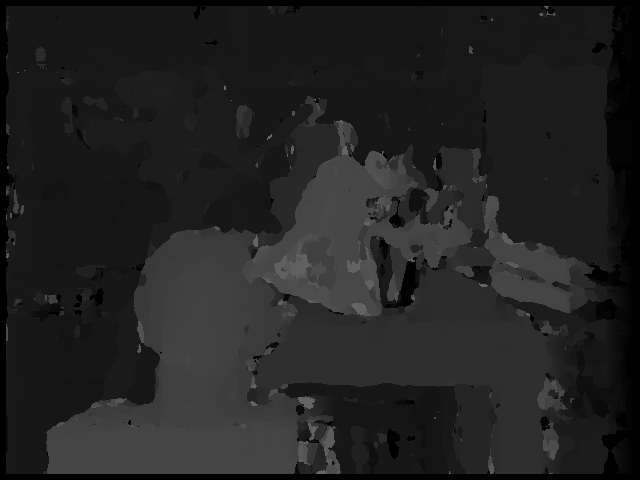
\includegraphics[width=.8\linewidth]{figures/CT9D0-100}
  \caption{9x9 census transform window \\Disparity range 0 to 100}
  \label{fig:sfig6}
\end{subfigure}
\begin{subfigure}{.5\textwidth}
  \centering
  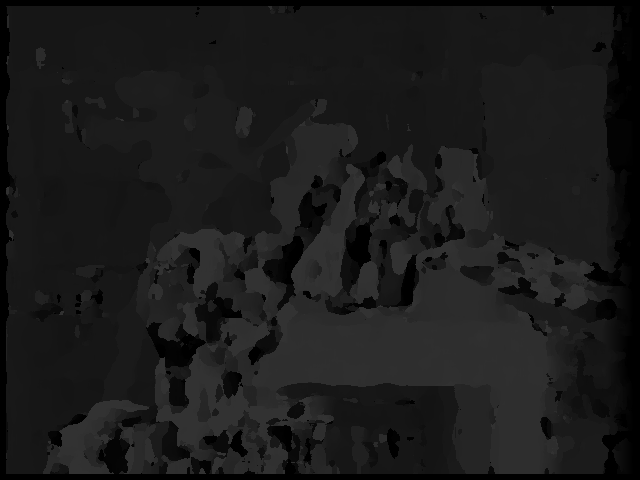
\includegraphics[width=.8\linewidth]{figures/CT11D0-50}
  \caption{11x11 census transform window \\Disparity range 0 to 50}
  \label{fig:sfig7}
\end{subfigure}%
\begin{subfigure}{.5\textwidth}
  \centering
  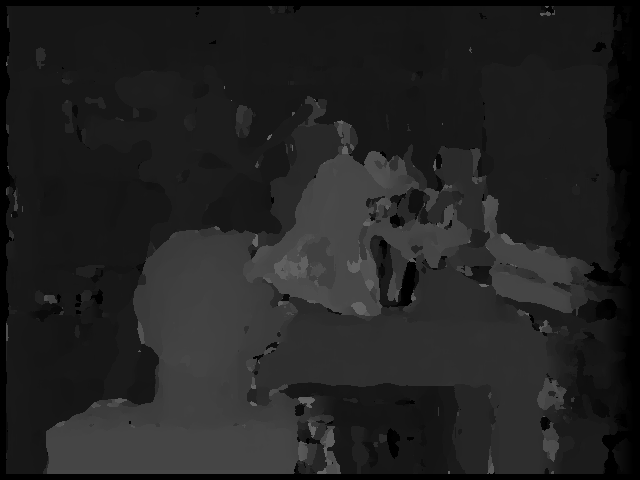
\includegraphics[width=.8\linewidth]{figures/CT11D0-100}
  \caption{11x11 census transform window \\Disparity range 0 to 100}
  \label{fig:sfig8}
\end{subfigure}
\caption{Disparity maps for Tsukuba image pair across different parameters}
\label{fig:dmappartsu}
\end{figure}


\begin{figure}
\captionsetup{justification=centering}
\captionsetup[subfigure]{justification=centering}
\begin{subfigure}{.5\textwidth}
  \centering
  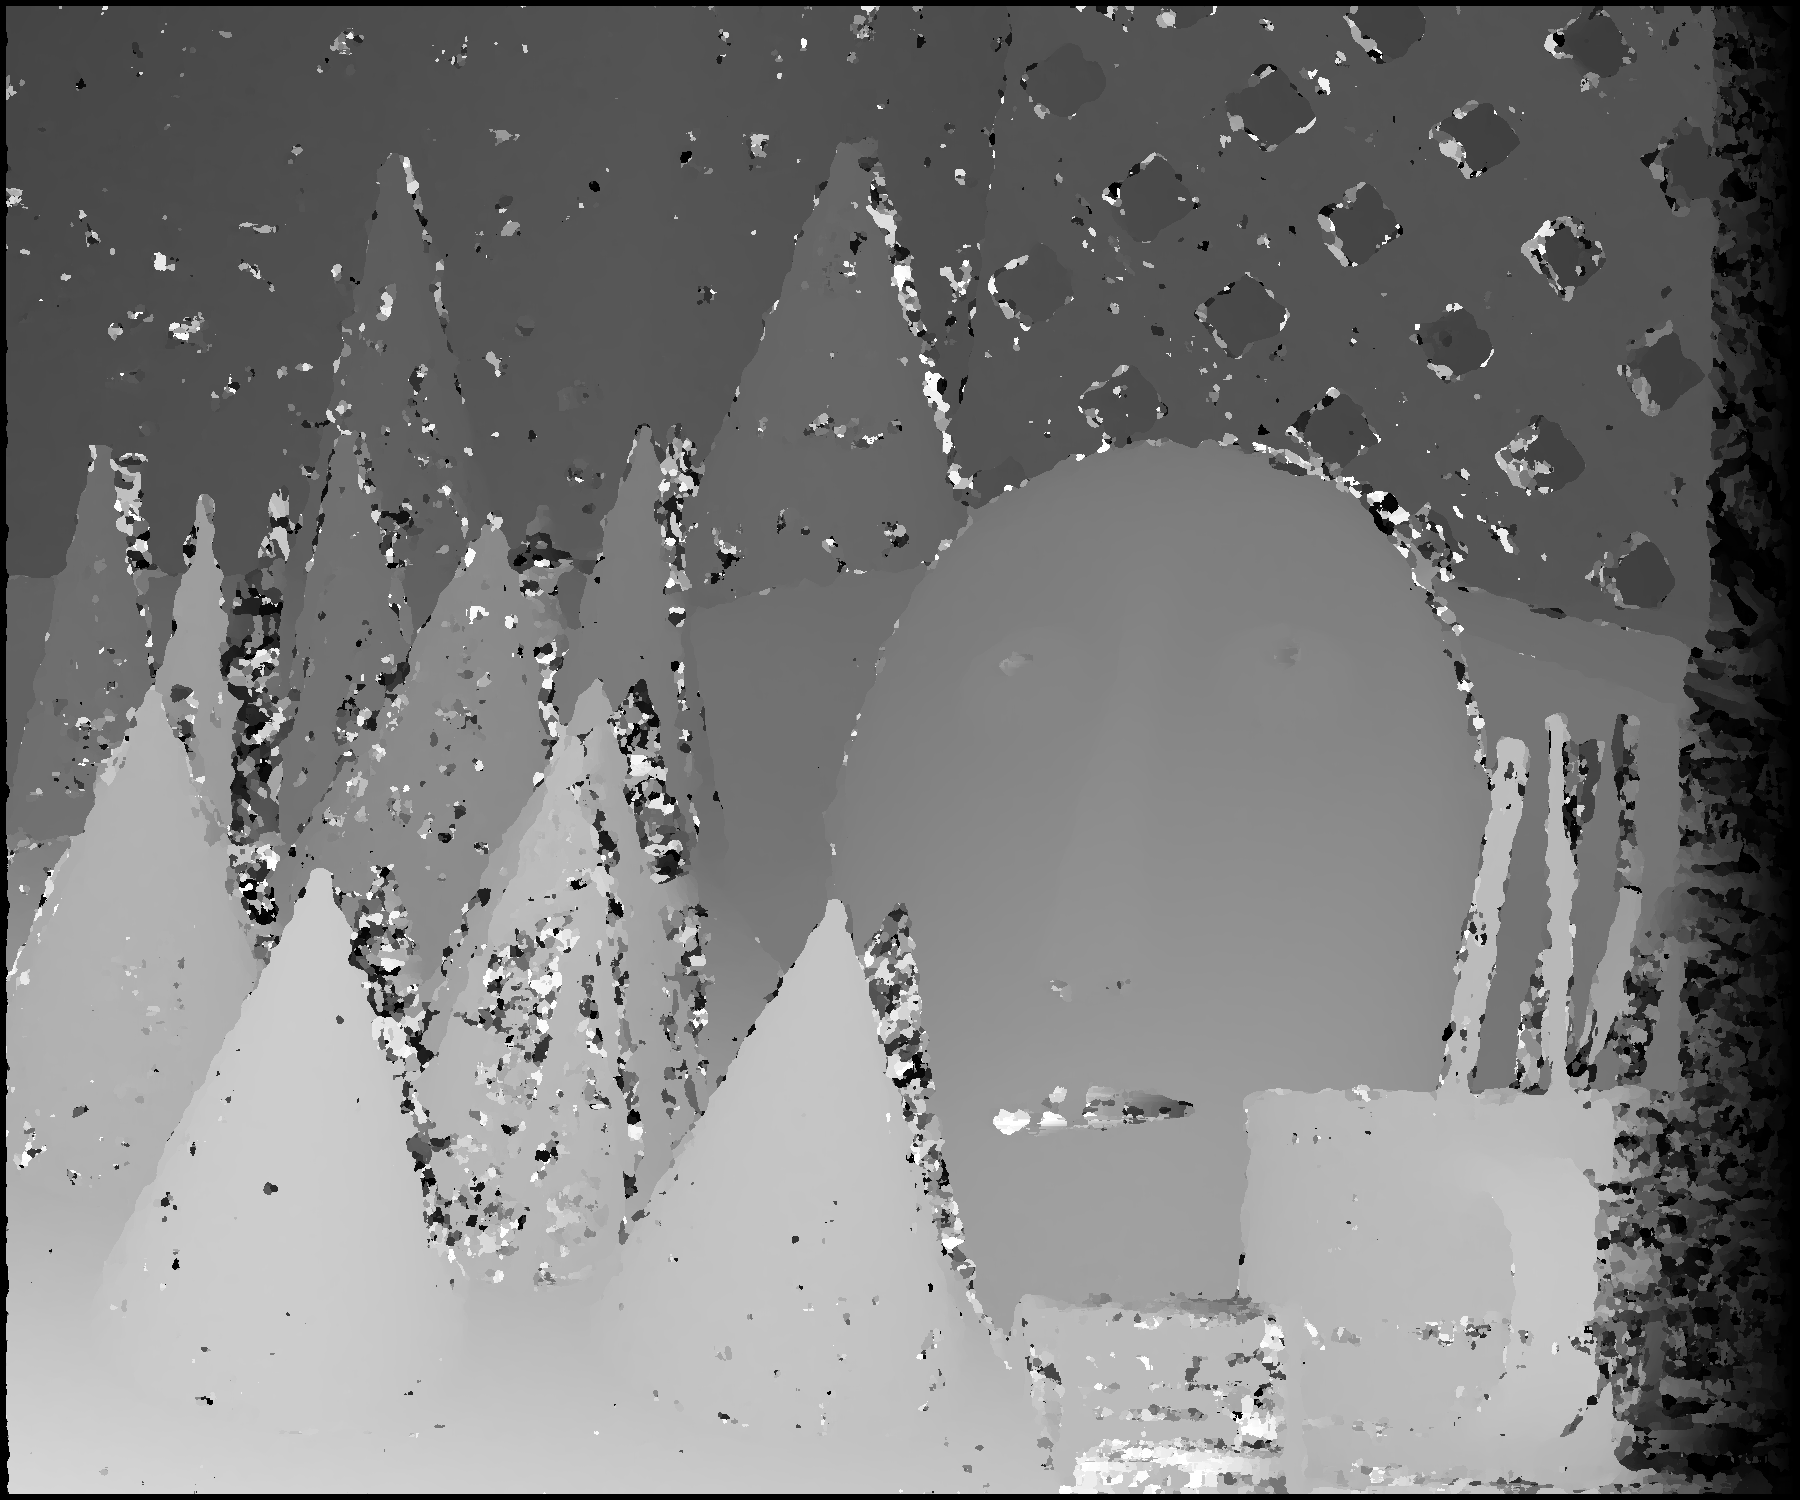
\includegraphics[width=.6\linewidth]{figures/ConeCT11D0-255}
  \caption{Disparity map}
  \label{fig:sfig1}
\end{subfigure}%
\begin{subfigure}{.5\textwidth}
  \centering
  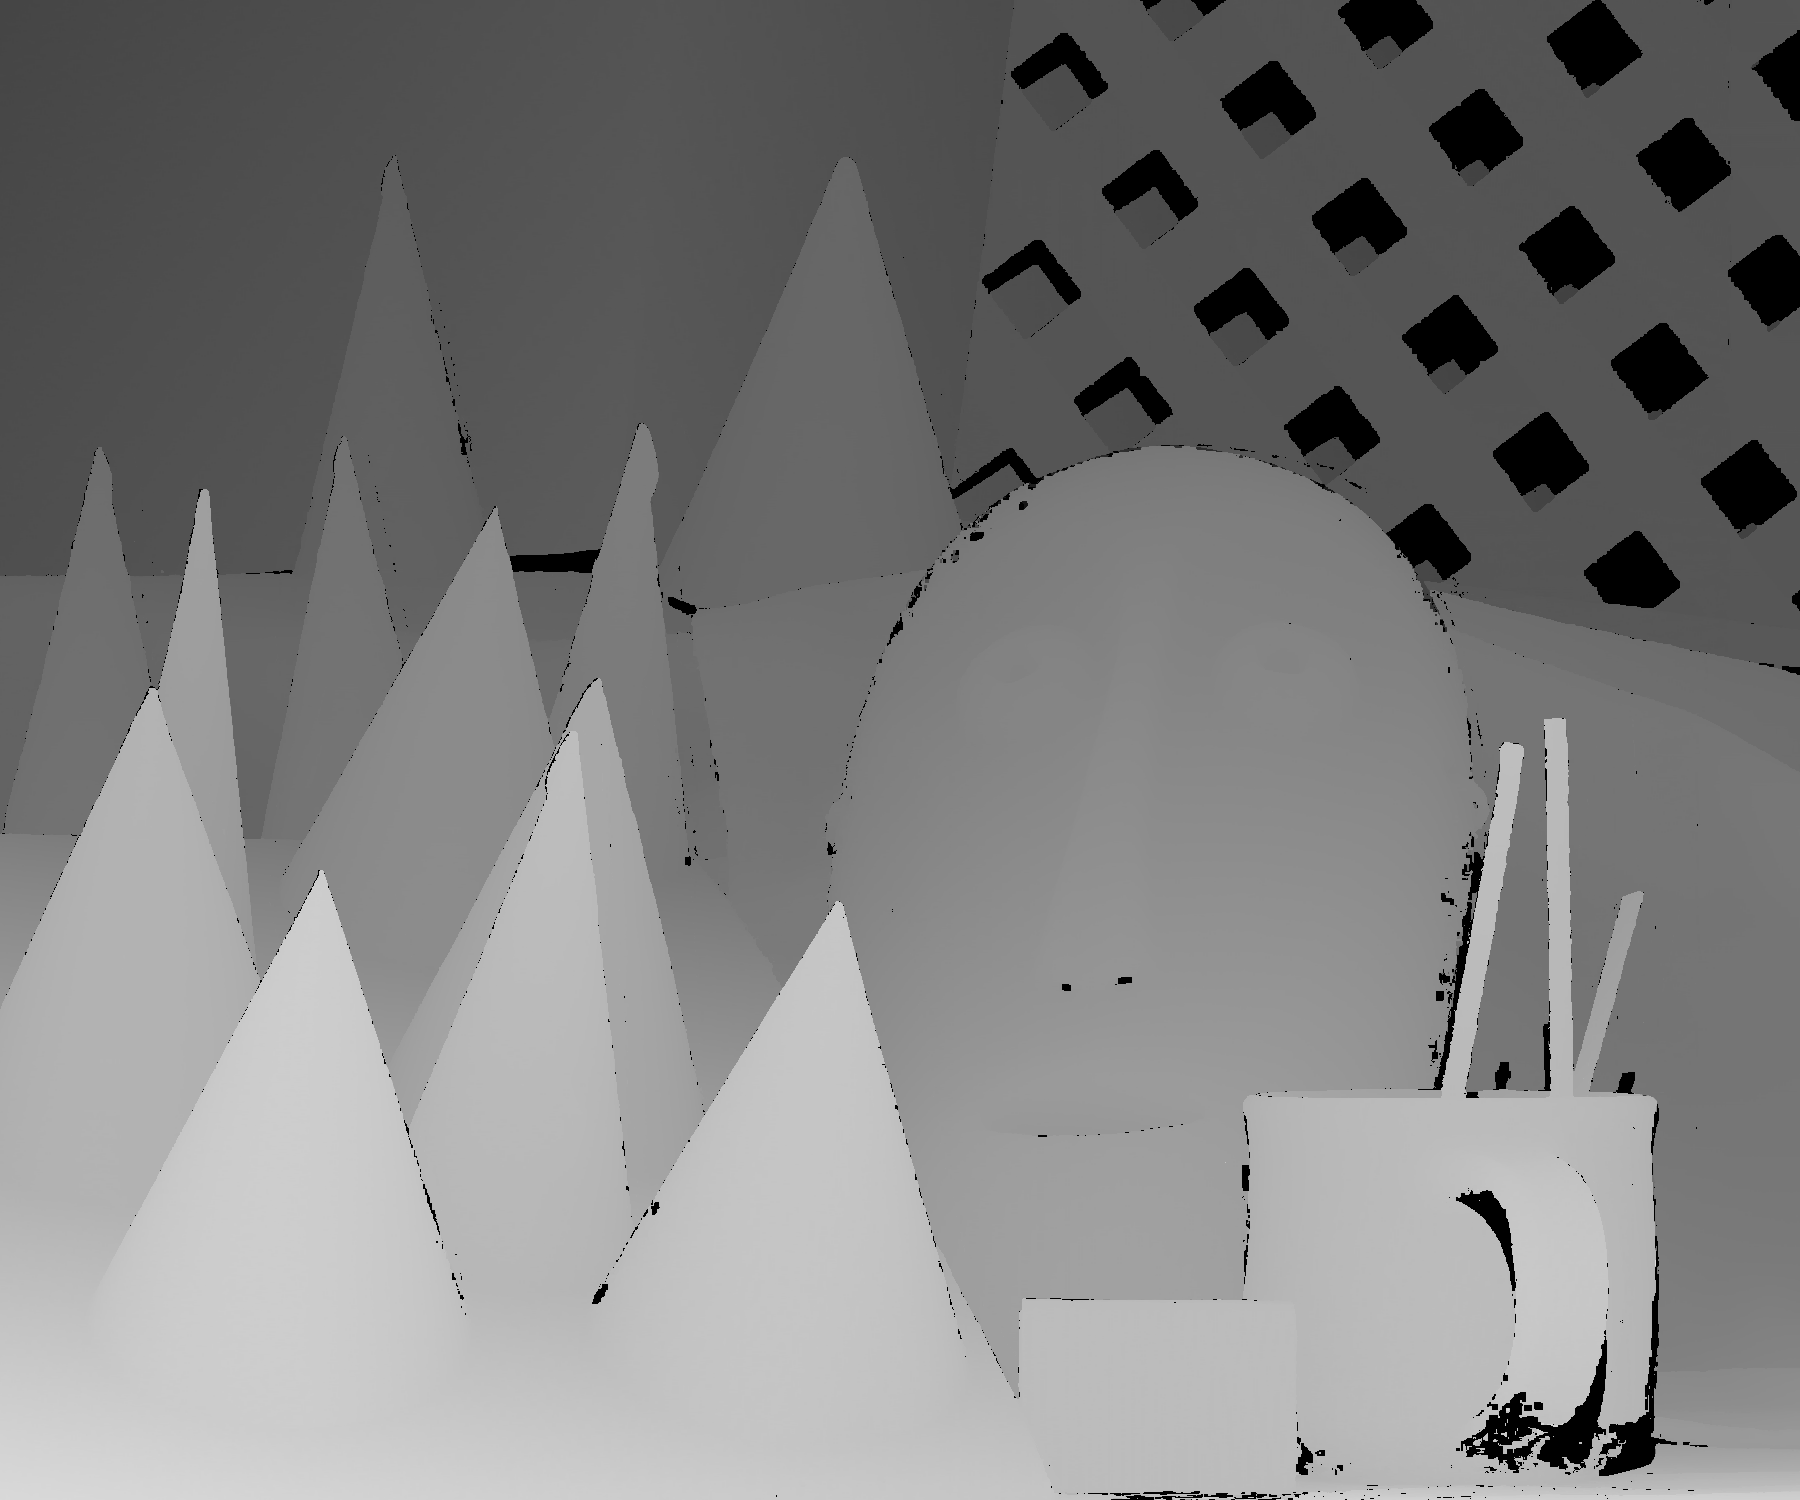
\includegraphics[width=.6\linewidth]{figures/ConeGT}
  \caption{Ground truth}
  \label{fig:sfig2}
\end{subfigure}
\caption{DM and ground truth for Cone(Middlebury) image pair with 11x11 census transform window and disparity range 0 to 255}
\label{fig:dmcone}
\end{figure}

% Please add the following required packages to your document preamble:
% \usepackage{booktabs}
\begin{table}[!htbp]
\centering
\begin{tabular}{@{}|c|c|c|c|c|c|@{}}
\toprule
\textbf{Image}        & \textbf{CT window size} & \textbf{Disp. Min.} & \textbf{Disp. Max} & \textbf{Resolution} & \textbf{BMPRE} \\ \midrule
Tsukuba frame 1       & 11                      & 0                   & 100                & 640x480             & 54800          \\ \midrule
Cone (Middlebury)     & 11                      & 0                   & 255                & 1800x1500           & 240000         \\ \midrule
Sawtooth (Middlebury) & 11                      & 0                   & 100                & 434x380             & 3161.3         \\ \bottomrule
\end{tabular}
\caption{BMPRE values ($\delta$=2) across images of different resolutions.}
\label{tab:bmpre}
\end{table}


The Figure \ref{fig:dmappartsu} shows the DM across different CTW and D range values for the Tsukuba university image pair along with the ground truth. The Table \ref{tab:bmpre} shows the BMPRE values (lower the better) across the images of different resolutions. The range of disparity values needs to be increased with resolution. This can be seen from the entry for Cone (Middlebury) in the table. Since that particular image pair is of high resolution, it requires greater number of disparity values for generating a detailed DM. The DM generated for the image pair can be seen in the Figure \ref{fig:dmcone}. It is also to be noted that BMPRE values probably increase with increase in resolution as more pixels are evaluated. This shows that the BMPRE values are not a global standard but depends on the resolution of the image.

\begin{figure}
  \center
  \captionsetup{justification=centering}
  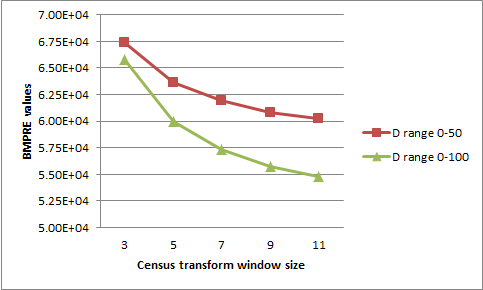
\includegraphics[width=.8\linewidth]{figures/BMPRE}
  \caption{BMPRE values across different CTW for different D ranges.}
  \label{fig:bmpre}
\end{figure}

 The effect of the window size and disparity range can be graphically seen in the Figure \ref{fig:bmpre}. This clearly shows the advantage of having larger census transform windows and greater range of disparity values. Census transform windows larger than 11 are not evaluated as it would require more than one data element(long integer) to store information for each pixel and might effectively nullify optimizations discussed in the Section \ref{sec:optimizations}.
 \\
From the observed results, the CTW value of 11 is chosen as it gives the best functional performance. D range of 0-100 is preferred as Tsukuba dataset is used, which is of resolution 640x480.

%%%%%%%%%%%%%%%%%%%%%%%%%
%%%%%   SUB-SECTION   %%%
%%%%%%%%%%%%%%%%%%%%%%%%%
%%%%%%%%%%%%%%%%%%%%%%%%%
\subsection{SHD window size (SHDW)}
\label{s:fverificationres:shdw}

\begin{figure}[!htbp]
  \center
  \captionsetup{justification=centering}
  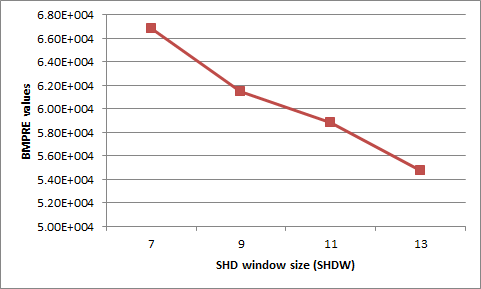
\includegraphics[width=.8\linewidth]{figures/BMPRE2}
  \caption{BMPRE values ($\delta$=2) across different SHDW values. Other parameters are kept constant with CTW=11, D range: 0-100, and MW=3}
  \label{fig:bmpre2}
\end{figure}

SHD calculation is a computational intensive calculation as it operates on a huge amount of data from the pre-processing stage. Census transformed (CTW=11) image yields 120 bits for every pixel in the image. SHDW plays an important role in determining the accuracy of DM. An experiment on the first frame from Tsukuba dataset across different SHDW values keeping the other parameters constant is performed. The results are as shown in the Figure \ref{fig:bmpre2}. It can be seen that SHDW value of 13 yields the best results for the tested values. Higher values of SHDW are not experimented owing to the computational intensity, which affects the execution time of the algorithm.

%%%%%%%%%%%%%%%%%%%%%%%%%%%%%%%%%%%%%
%%%%%%%%%%%%%%%%%%%%%%%%%%%%%%%%%%%%%
%%%%%%%%%%%%   SECTION   %%%%%%%%%%%%
%%%%%%%%%%%%%%%%%%%%%%%%%%%%%%%%%%%%%
%%%%%%%%%%%%%%%%%%%%%%%%%%%%%%%%%%%%%
\section{Algorithm run-time performance}

% Please add the following required packages to your document preamble:
% \usepackage{booktabs}
\begin{table}[!htbp]
\centering
\begin{tabular}{@{}|c|c|c|c|c|@{}}
\toprule
\textbf{Hardware}    & \textbf{RAM (GB)} & \textbf{Clock(GHz)} & \textbf{Cores} & \textbf{Threads} \\ \midrule
Intel Core i3-350M   & 3                 & 2.26                & 2              & 4                \\ \midrule
Intel Core i5-2500K  & 16                & 3.3                 & 4              & 4                \\ \midrule
Intel Core i7-5820K* & 32                & 3.3                 & 6              & 6                \\ \bottomrule
\end{tabular}
\captionsetup{justification=centering}
\caption{Hardware platform details. \\ *It is to be noted that Intel Corei7 was implemented using virtual machine.}
\label{tab:hwplat}
\end{table}

In this section, various optimized versions of algorithm discussed in the Section \ref{sec:optimizations} is evaluated for execution time across different hardware. The Table \ref{tab:hwplat} shows the details of the hardware platforms. Linux OS with the 3.13.0-85-generic kernel is used for implementation. A single frame-pair from the Tsukuba dataset is evaluated for the purpose. The versions of the algorithm are numbered as shown in Figure \ref{fig:algover} according to the optimizations involved. Optimizations which do not yield favourable results are avoided in the subsequent versions of the algorithm. The performance of algorithm across different hardware is as shown in the Figure \ref{fig:algort}.

\begin{figure}[!htbp]
    \center
    \captionsetup{justification=centering}
    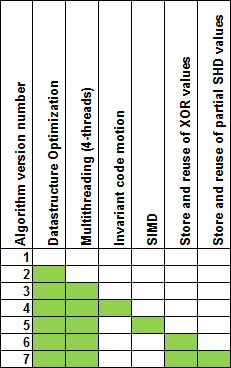
\includegraphics[width=.4\linewidth]{figures/AlgoVersions}
    \caption{Various versions of algorithm with the optimizations involved.}
    \label{fig:algover}
\end{figure}

\begin{figure}[!htbp]
    \center
    \captionsetup{justification=centering}
    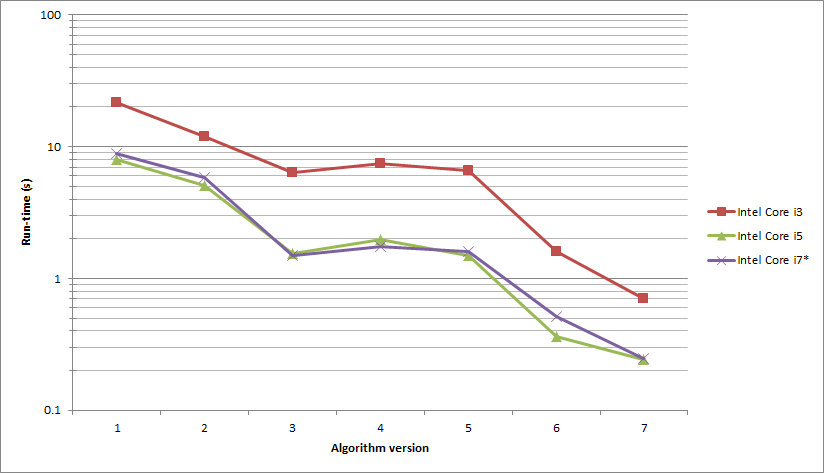
\includegraphics[width=\linewidth]{figures/Runtime}
    \caption{Runtime of various versions of algorithm across different hardware.\\ *It is to be noted that performance in Intel Corei7 was measured using virtual machine and hence might be relatively slower than actual performance}
    \label{fig:algort}
\end{figure}

The numbers shown in the Figure \ref{fig:algort} are from the C++ implementation of the algorithm in Linux with gcc 4.9.3 compiler. The values are obtained by running the algorithm 10 times and averaging the results in each case. The figure shows that algorithm performs better in Intel Corei5 and i7 compared to i3. This is due to the presence of more cores as indicated by the Table \ref{tab:hwplat} and hence better support for multi-threading. As indicated in the figure there does not seem to be much of speed up achieved in i7 implementation against i5, probably due to the fact that the i7 measurements were taken using a virtual machine, VMware.\\

From the figure, it can be seen that the optimizations Invariant code motion and  SIMD do not yeild favourable results. The reason for slower perfomance with Invariant code motion might probably be due to register spill as multiple threads are involved in executing the same code. SIMD optimization, as discussed in the Section \ref{s:optimizations:simd}, involves parallelizing the XOR calculation in SHD calculation. However, SHD calculation also involves calculating the bit count which cannot be sped-up using SIMD. This reduces the speed-up that can be achieved. Also the register spill discussed in the Section \ref{s:optimizations:invariantcodemotion} might come into play in this case as well due to multiple threads, thus resulting in a slow-down of the algorithm's performance.\\

The numbers indicated in the Figure \ref{fig:algort} are processing times, which exclude the time taken for the input of the image. An analysis done on the pre-processing time(Census transform), total processing time(SHD and pre-processing), and total program run-time reveals the following, for most optimized version of algorithm:
\begin{itemize}
\item{The inupt and output of images take about 15\% of the run time. This time would be replaced by the reading time from the camera and writing time to frame buffer in a real application. It is safe to assume that this time might not accumulate with every frame, but might result in a delay in output as dedicated hardware is involved.}
\item{The pre-processing takes about 48\% of the processing time. Most of the optimizations discussed in the Section \ref{sec:optimizations} involve optimizing the SHD part of the algorithm. Further research in optimizing the pre-processing part will effectively result in faster execution of the algorithm.}
\item{The most optimized version of the algorithm executes 31X, 32X and 35X faster than the unoptimized version in Intel core i3,i5 and i7 respectively.}
\item{The fastest execution time of the algorithm in any of the tested hardware is 0.2427636s for one frame. This is still 5 times slower than the execution time expected for real-time operation(20 fps). This suggests that further acceleration, is required for real-time operation.}
\end{itemize}

%%%%%%%%%%%%%%%%%%%%%%%%%%%%%%%%%%%%%
%%%%%%%%%%%%%%%%%%%%%%%%%%%%%%%%%%%%%
%%%%%%%%%%%%   SECTION   %%%%%%%%%%%%
%%%%%%%%%%%%%%%%%%%%%%%%%%%%%%%%%%%%%
%%%%%%%%%%%%%%%%%%%%%%%%%%%%%%%%%%%%%
\section{Summary}
This chapter discussed on the method used for functional verification. The important parameters of the algorithm were discussed. The functional performance of the algorithm across different parameters was persented. MW of 3, CTW of 11, D range of 0-100 and SHDW of 13 were chosen for implementation in Nema. Subsequently, the execution time of the algorithm across various hardware was presented and valid optimizations were chosen. Valid optimizations provide 31X to 35X speed up based on the hardware implemented. Further observations were recorded.